\documentclass[]{article}
    %%%%%%%%%%%%%%%%%%%%%%%%%%%%%%%%%%%%%%%%%
% Lachaise Assignment
% Structure Specification File
% Version 1.0 (26/6/2018)
%
% This template originates from:
% http://www.LaTeXTemplates.com
%
% Authors:
% Marion Lachaise & François Févotte
% Vel (vel@LaTeXTemplates.com)
%
% License:
% CC BY-NC-SA 3.0 (http://creativecommons.org/licenses/by-nc-sa/3.0/)
% 
%%%%%%%%%%%%%%%%%%%%%%%%%%%%%%%%%%%%%%%%%

%----------------------------------------------------------------------------------------
%	PACKAGES AND OTHER DOCUMENT CONFIGURATIONS
%----------------------------------------------------------------------------------------

\usepackage{amsmath,amsfonts,stmaryrd,amssymb} % Math packages

\usepackage{enumerate} % Custom item numbers for enumerations

\usepackage[ruled]{algorithm2e} % Algorithms

\usepackage[framemethod=tikz]{mdframed} % Allows defining custom boxed/framed environments

\usepackage{listings} % File listings, with syntax highlighting
\lstset{
	basicstyle=\ttfamily, % Typeset listings in monospace font
}

%----------------------------------------------------------------------------------------
%	DOCUMENT MARGINS
%----------------------------------------------------------------------------------------

\usepackage{geometry} % Required for adjusting page dimensions and margins

\geometry{
	paper=a4paper, % Paper size, change to letterpaper for US letter size
	top=2.5cm, % Top margin
	bottom=3cm, % Bottom margin
	left=2.5cm, % Left margin
	right=2.5cm, % Right margin
	headheight=14pt, % Header height
	footskip=1.5cm, % Space from the bottom margin to the baseline of the footer
	headsep=1.2cm, % Space from the top margin to the baseline of the header
	% showframe, % Uncomment to show how the type block is set on the page
}

%----------------------------------------------------------------------------------------
%	FONTS
%----------------------------------------------------------------------------------------

\usepackage[utf8]{inputenc} % Required for inputting international characters
\usepackage[T1]{fontenc} % Output font encoding for international characters

% \usepackage{XCharter} % Use the XCharter fonts\usepackage{XCharter} % Use the XCharter fonts

%----------------------------------------------------------------------------------------
%	COMMAND LINE ENVIRONMENT
%----------------------------------------------------------------------------------------

% Usage:
% \begin{commandline}
%	\begin{verbatim}
%		$ ls
%		
%		Applications	Desktop	...
%	\end{verbatim}
% \end{commandline}

\mdfdefinestyle{commandline}{
	leftmargin=10pt,
	rightmargin=10pt,
	innerleftmargin=15pt,
	middlelinecolor=black!50!white,
	middlelinewidth=2pt,
	frametitlerule=false,
	backgroundcolor=black!5!white,
	frametitle={Command Line},
	frametitlefont={\normalfont\sffamily\color{white}\hspace{-1em}},
	frametitlebackgroundcolor=black!50!white,
	nobreak,
}

% Define a custom environment for command-line snapshots
\newenvironment{commandline}{
	\medskip
	\begin{mdframed}[style=commandline]
}{
	\end{mdframed}
	\medskip
}

%----------------------------------------------------------------------------------------
%	FILE CONTENTS ENVIRONMENT
%----------------------------------------------------------------------------------------

% Usage:
% \begin{file}[optional filename, defaults to "File"]
%	File contents, for example, with a listings environment
% \end{file}

\mdfdefinestyle{file}{
	innertopmargin=1.6\baselineskip,
	innerbottommargin=0.8\baselineskip,
	topline=false, bottomline=false,
	leftline=false, rightline=false,
	leftmargin=1cm,
	rightmargin=1cm,
	singleextra={%
		\draw[fill=black!10!white](P)++(0,-1.2em)rectangle(P-|O);
		\node[anchor=north west]
		at(P-|O){\ttfamily\mdfilename};
		%
		\def\l{3em}
		\draw(O-|P)++(-\l,0)--++(\l,\l)--(P)--(P-|O)--(O)--cycle;
		\draw(O-|P)++(-\l,0)--++(0,\l)--++(\l,0);
	},
	nobreak,
}

% Define a custom environment for file contents
\newenvironment{file}[1][File]{ % Set the default filename to "File"
	\medskip
	\newcommand{\mdfilename}{#1}
	\begin{mdframed}[style=file]
}{
	\end{mdframed}
	\medskip
}

%----------------------------------------------------------------------------------------
%	NUMBERED QUESTIONS ENVIRONMENT
%----------------------------------------------------------------------------------------

% Usage:
% \begin{question}[optional title]
%	Question contents
% \end{question}

\mdfdefinestyle{question}{
	innertopmargin=1.2\baselineskip,
	innerbottommargin=0.8\baselineskip,
	roundcorner=5pt,
	nobreak,
	singleextra={%
		\draw(P-|O)node[xshift=1em,anchor=west,fill=white,draw,rounded corners=5pt]{%
		Question \theQuestion\questionTitle};
	},
}

\newcounter{Question} % Stores the current question number that gets iterated with each new question

% Define a custom environment for numbered questions
\newenvironment{question}[1][\unskip]{
	\bigskip
	\stepcounter{Question}
	\newcommand{\questionTitle}{~#1}
	\begin{mdframed}[style=question]
}{
	\end{mdframed}
	\medskip
}

%----------------------------------------------------------------------------------------
%	WARNING TEXT ENVIRONMENT
%----------------------------------------------------------------------------------------

% Usage:
% \begin{warn}[optional title, defaults to "Warning:"]
%	Contents
% \end{warn}

\mdfdefinestyle{warning}{
	topline=false, bottomline=false,
	leftline=false, rightline=false,
	nobreak,
	singleextra={%
		\draw(P-|O)++(-0.5em,0)node(tmp1){};
		\draw(P-|O)++(0.5em,0)node(tmp2){};
		\fill[black,rotate around={45:(P-|O)}](tmp1)rectangle(tmp2);
		\node at(P-|O){\color{white}\scriptsize\bf !};
		\draw[very thick](P-|O)++(0,-1em)--(O);%--(O-|P);
	}
}

% Define a custom environment for warning text
\newenvironment{warn}[1][Warning:]{ % Set the default warning to "Warning:"
	\medskip
	\begin{mdframed}[style=warning]
		\noindent{\textbf{#1}}
}{
	\end{mdframed}
}

%----------------------------------------------------------------------------------------
%	INFORMATION ENVIRONMENT
%----------------------------------------------------------------------------------------

% Usage:
% \begin{info}[optional title, defaults to "Info:"]
% 	contents
% 	\end{info}

\mdfdefinestyle{info}{%
	topline=false, bottomline=false,
	leftline=false, rightline=false,
	nobreak,
	singleextra={%
		\fill[black](P-|O)circle[radius=0.4em];
		\node at(P-|O){\color{white}\scriptsize\bf i};
		\draw[very thick](P-|O)++(0,-0.8em)--(O);%--(O-|P);
	}
}

% Define a custom environment for information
\newenvironment{info}[1][Info:]{ % Set the default title to "Info:"
	\medskip
	\begin{mdframed}[style=info]
		\noindent{\textbf{#1}}
}{
	\end{mdframed}
}

    \usepackage{fontspec}
    \usepackage{indentfirst}
    \usepackage{booktabs}
    \setmainfont{思源宋体 CN}
    \XeTeXlinebreaklocale "zh"
    \XeTeXlinebreakskip = 0pt plus 1pt

    \title{Computer Vision 2018 Fall Assignment \\ \textbf{\#1 Camera Calibration}}
    \author{张义飞 --- 201821080630\\ \texttt{yidadaa@qq.com}}
    \date{\small{UESTC --- \today}}
    
    \begin{document}

    \maketitle

    \section{相机标定简介}
    在图像测量过程以及机器视觉应用中,为确定空间物体表面某点的三维几何位置与其在图像中对应点之间的相互关系,必须建立相机成像的几何模型,这些几何模型参数就是相机参数。\\
    
    在大多数条件下这些参数必须通过实验与计算才能得到,这个求解参数(内参、外参、畸变参数)的过程就称之为\textbf{相机标定}(或摄像机标定)。无论是在图像测量或者机器视觉应用中,相机参数的标定都是非常关键的环节,其标定结果的精度及算法的稳定性直接影响相机工作产生结果的准确性。因此,做好相机标定是做好后续工作的前提,提高标定精度是科研工作的重点所在。\\
    
    \begin{question}
        明确相机标定任务的内容。
        \begin{enumerate}
            \item \textbf{目的:}获取摄像机的内参和外参矩阵(同时也会得到每一幅标定图像的选择和平移矩阵),内参和外参系数可以对之后相机拍摄的图像就进行矫正,得到畸变相对很小的图像。
            \item \textbf{输入:}标定图像上所有内角点的图像坐标,标定板图像上所有内角点的空间三维坐标(一般情况下假定图像位于Z=0平面上)。
            \item \textbf{输出:}摄像机的内参、外参系数。
        \end{enumerate}
    \end{question}

    \section{具体实现}
    本报告使用opencv自带的张正友相机标定法进行标定,标定流程如下所示:
    \begin{enumerate}
        \item 准备标定图片;
        \item 提取标定图片中的角点信息以及亚像素信息;
        \item 执行相机标定;
        \item 计算误差,评价标定结果;
        \item 使用标定结果,对原图做矫正。
    \end{enumerate}

    本节将一步一步执行上述的标定流程,并将每一步的结果展示出来。
    \subsection{准备标定图片并提取角点信息}
    OpenCV使用棋盘格板进行标定,为了标定相机,我们需要输入一系列三维点和它们对应的二维图像点。在黑白相间的棋盘格上,二维图像点很容易通过角点检测找到。而对于真实世界中的三维点呢?由于我们采集中,是将相机放在一个地方,而将棋盘格定标板进行移动变换不同的位置,然后对其进行拍摄。\\
    
    所以我们需要知道(X,Y,Z)的值。但是简单来说,我们定义棋盘格所在平面为XY平面,即Z=0。对于定标板来说,我们可以知道棋盘格的方块尺寸,例如30mm,这样我们就可以把棋盘格上的角点坐标定义为(0,0,0),(30,0,0),(60,0,0),···,这个结果的单位是mm。3D点称为Object Points,2D图像点称为Image Points。

    \begin{figure}[htbp]
        \centering
        \begin{minipage}[t]{0.4\textwidth}
            \centering
            \includegraphics[width=6cm]{../code/images/0.jpg}
        \end{minipage}
        \begin{minipage}[t]{0.4\textwidth}
            \centering
            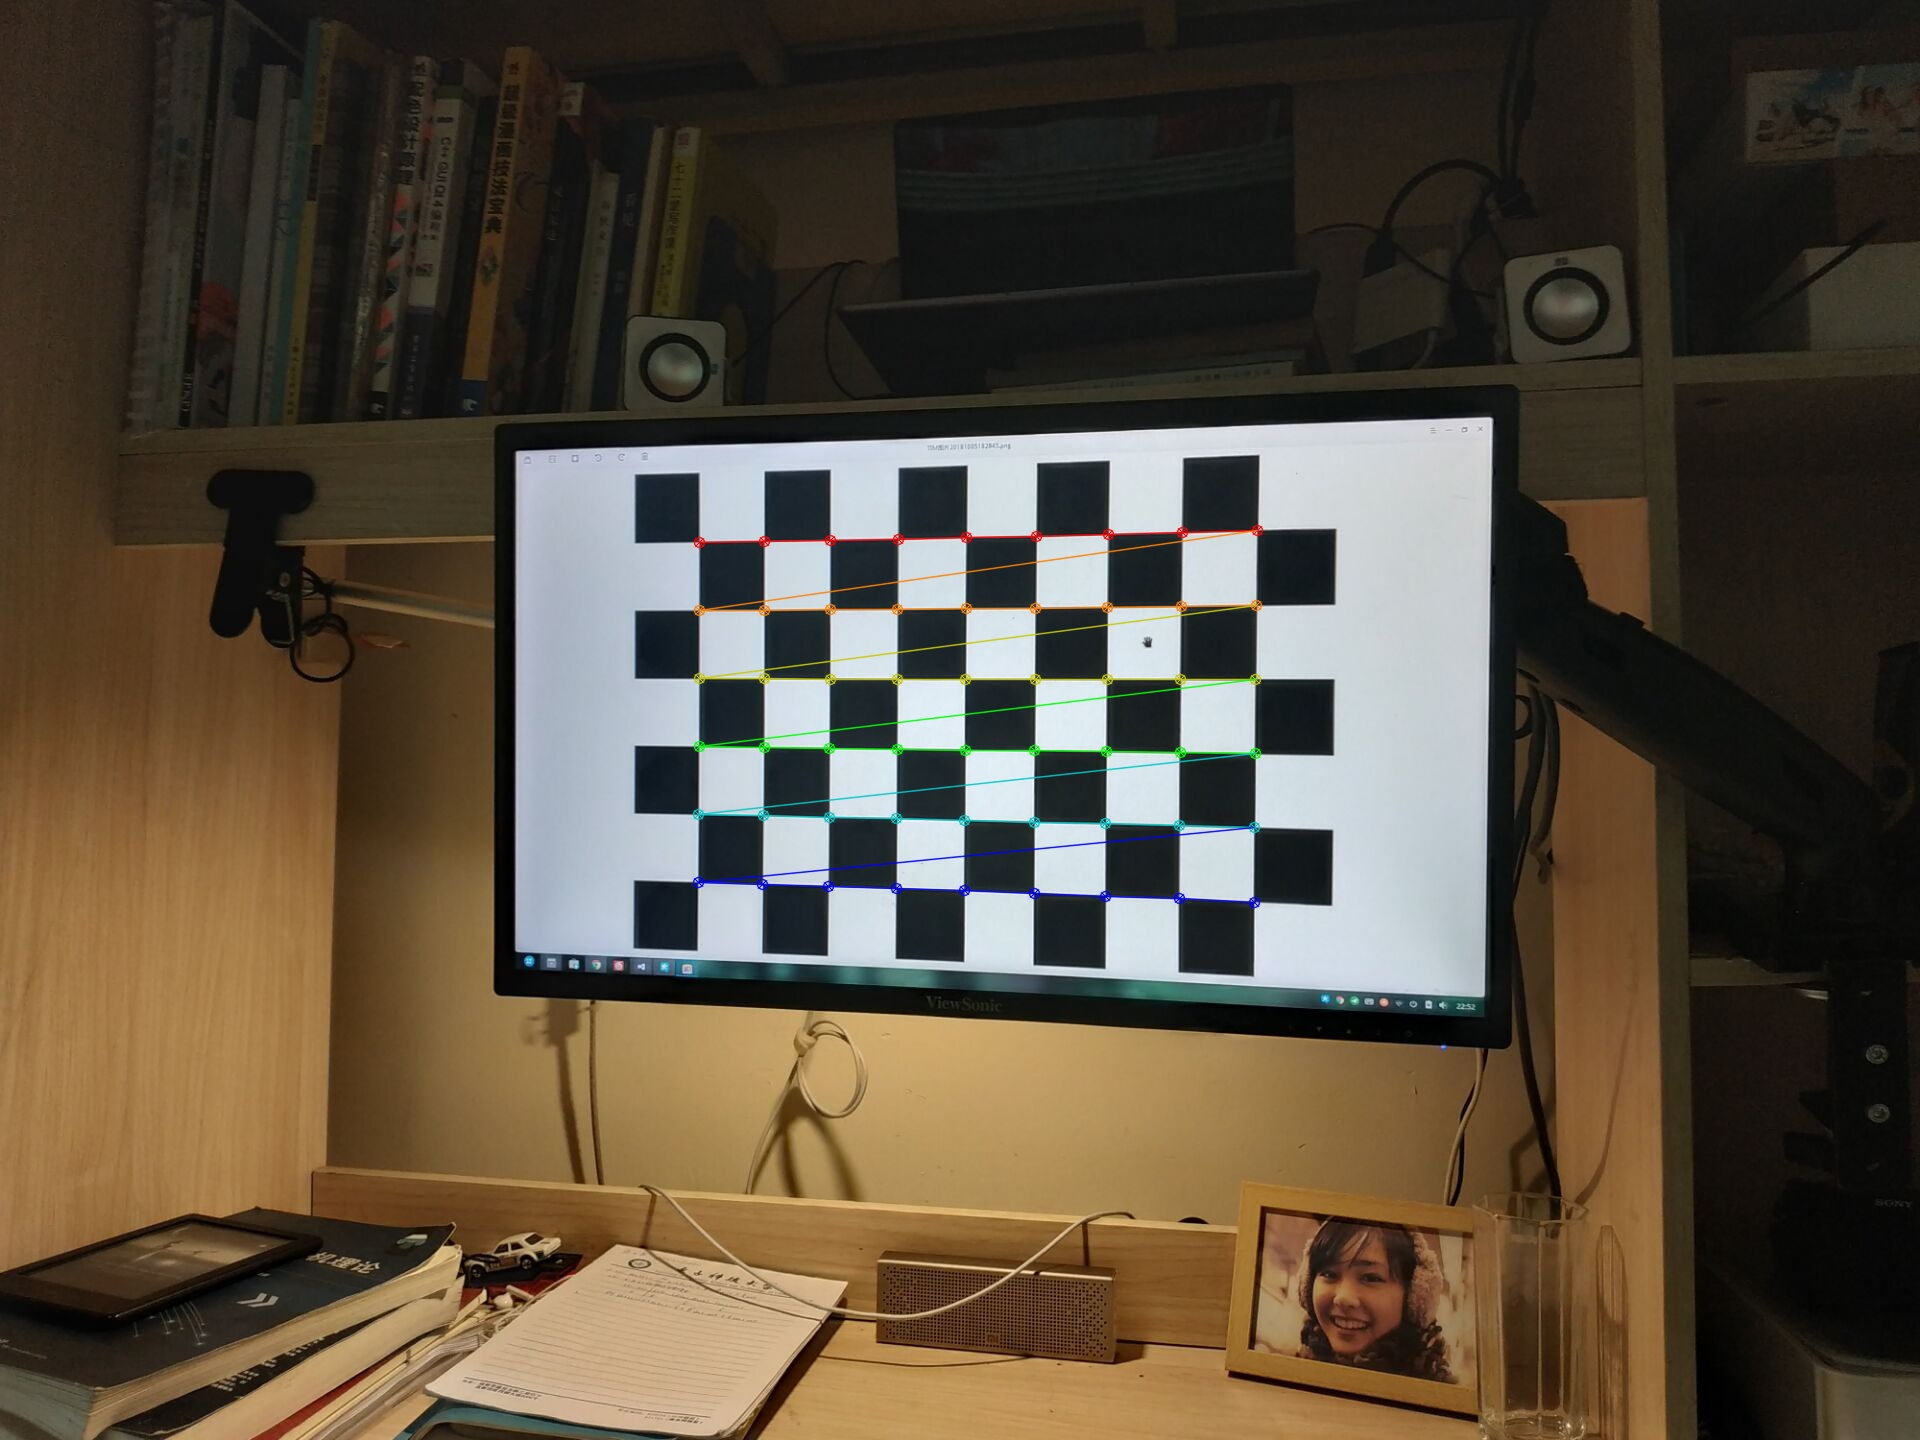
\includegraphics[width=6cm]{../code/images/0_jpg_with_corners.jpg}
        \end{minipage}

        \begin{minipage}[t]{0.4\textwidth}
            \centering
            \includegraphics[width=6cm]{../code/images/1.jpg}
        \end{minipage}
        \begin{minipage}[t]{0.4\textwidth}
            \centering
            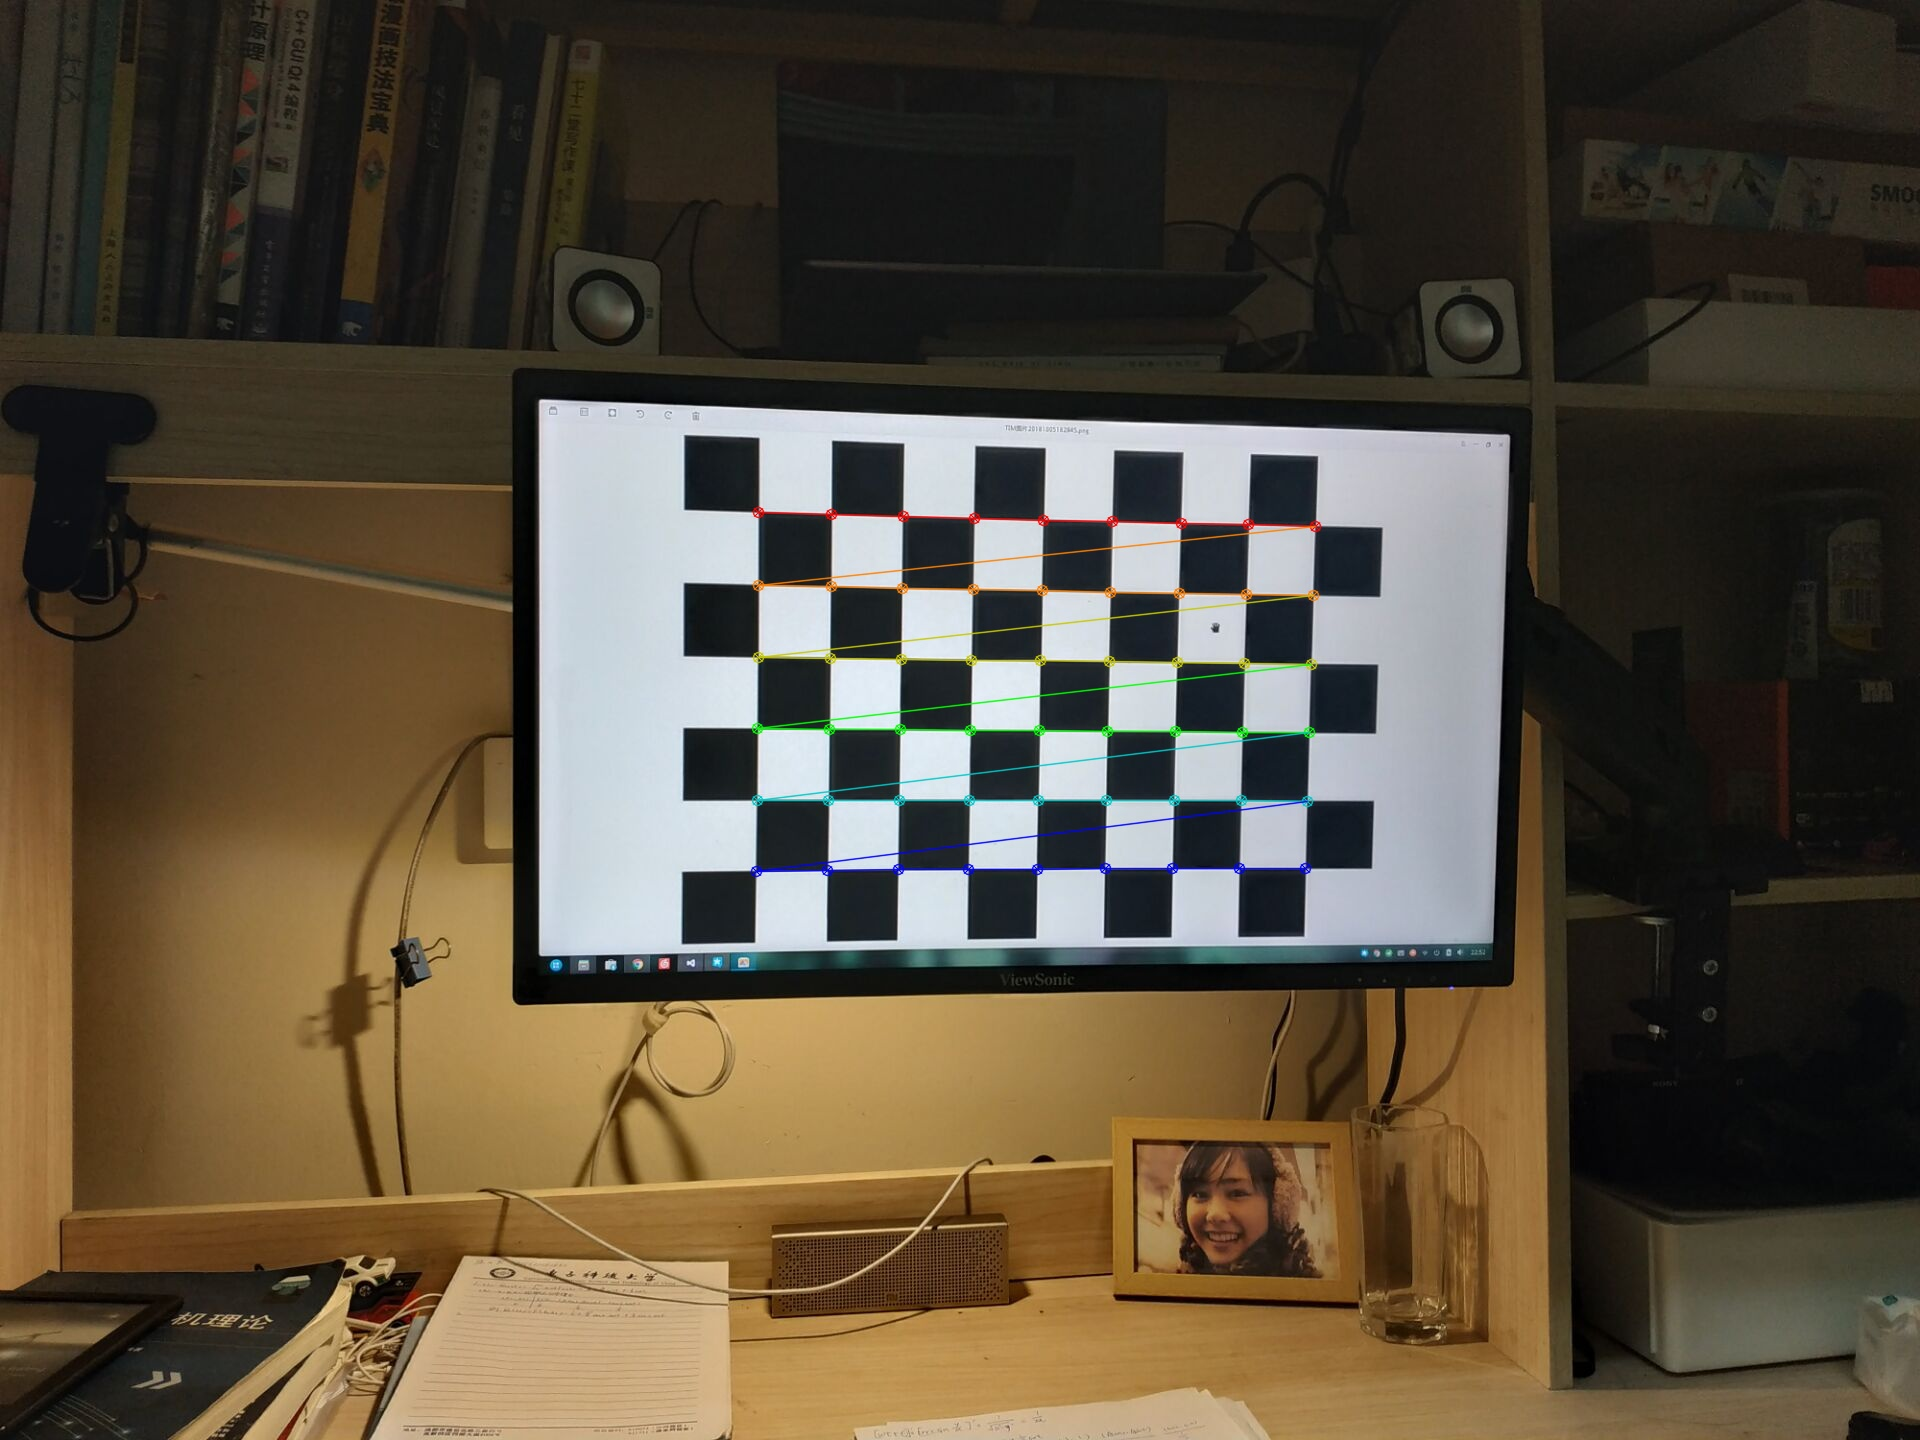
\includegraphics[width=6cm]{../code/images/1_jpg_with_corners.jpg}
        \end{minipage}

        \begin{minipage}[t]{0.4\textwidth}
            \centering
            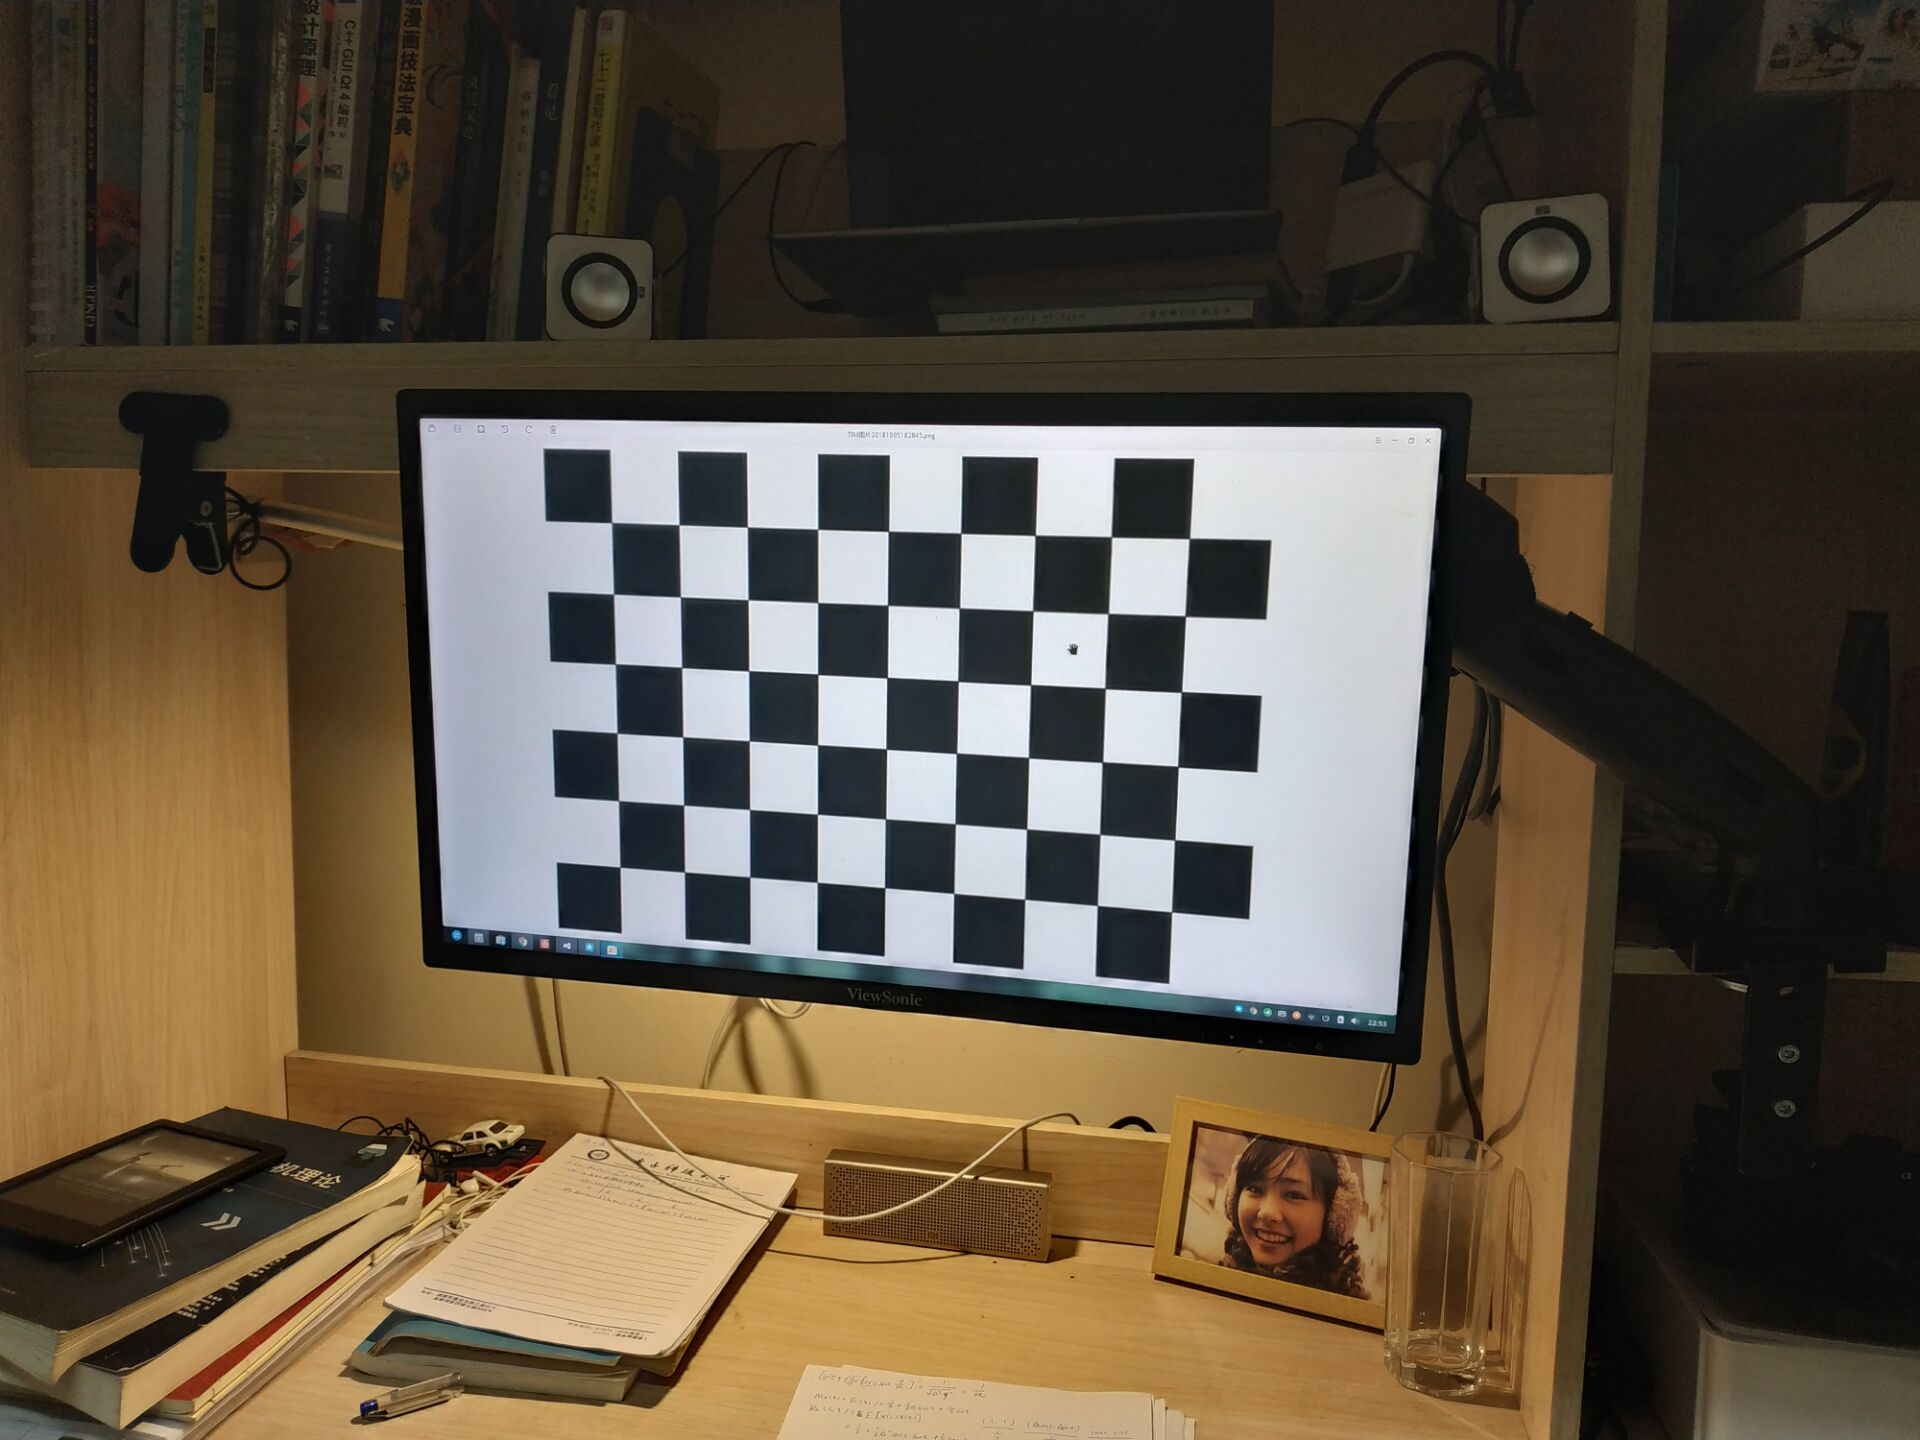
\includegraphics[width=6cm]{../code/images/2.jpg}
        \end{minipage}
        \begin{minipage}[t]{0.4\textwidth}
            \centering
            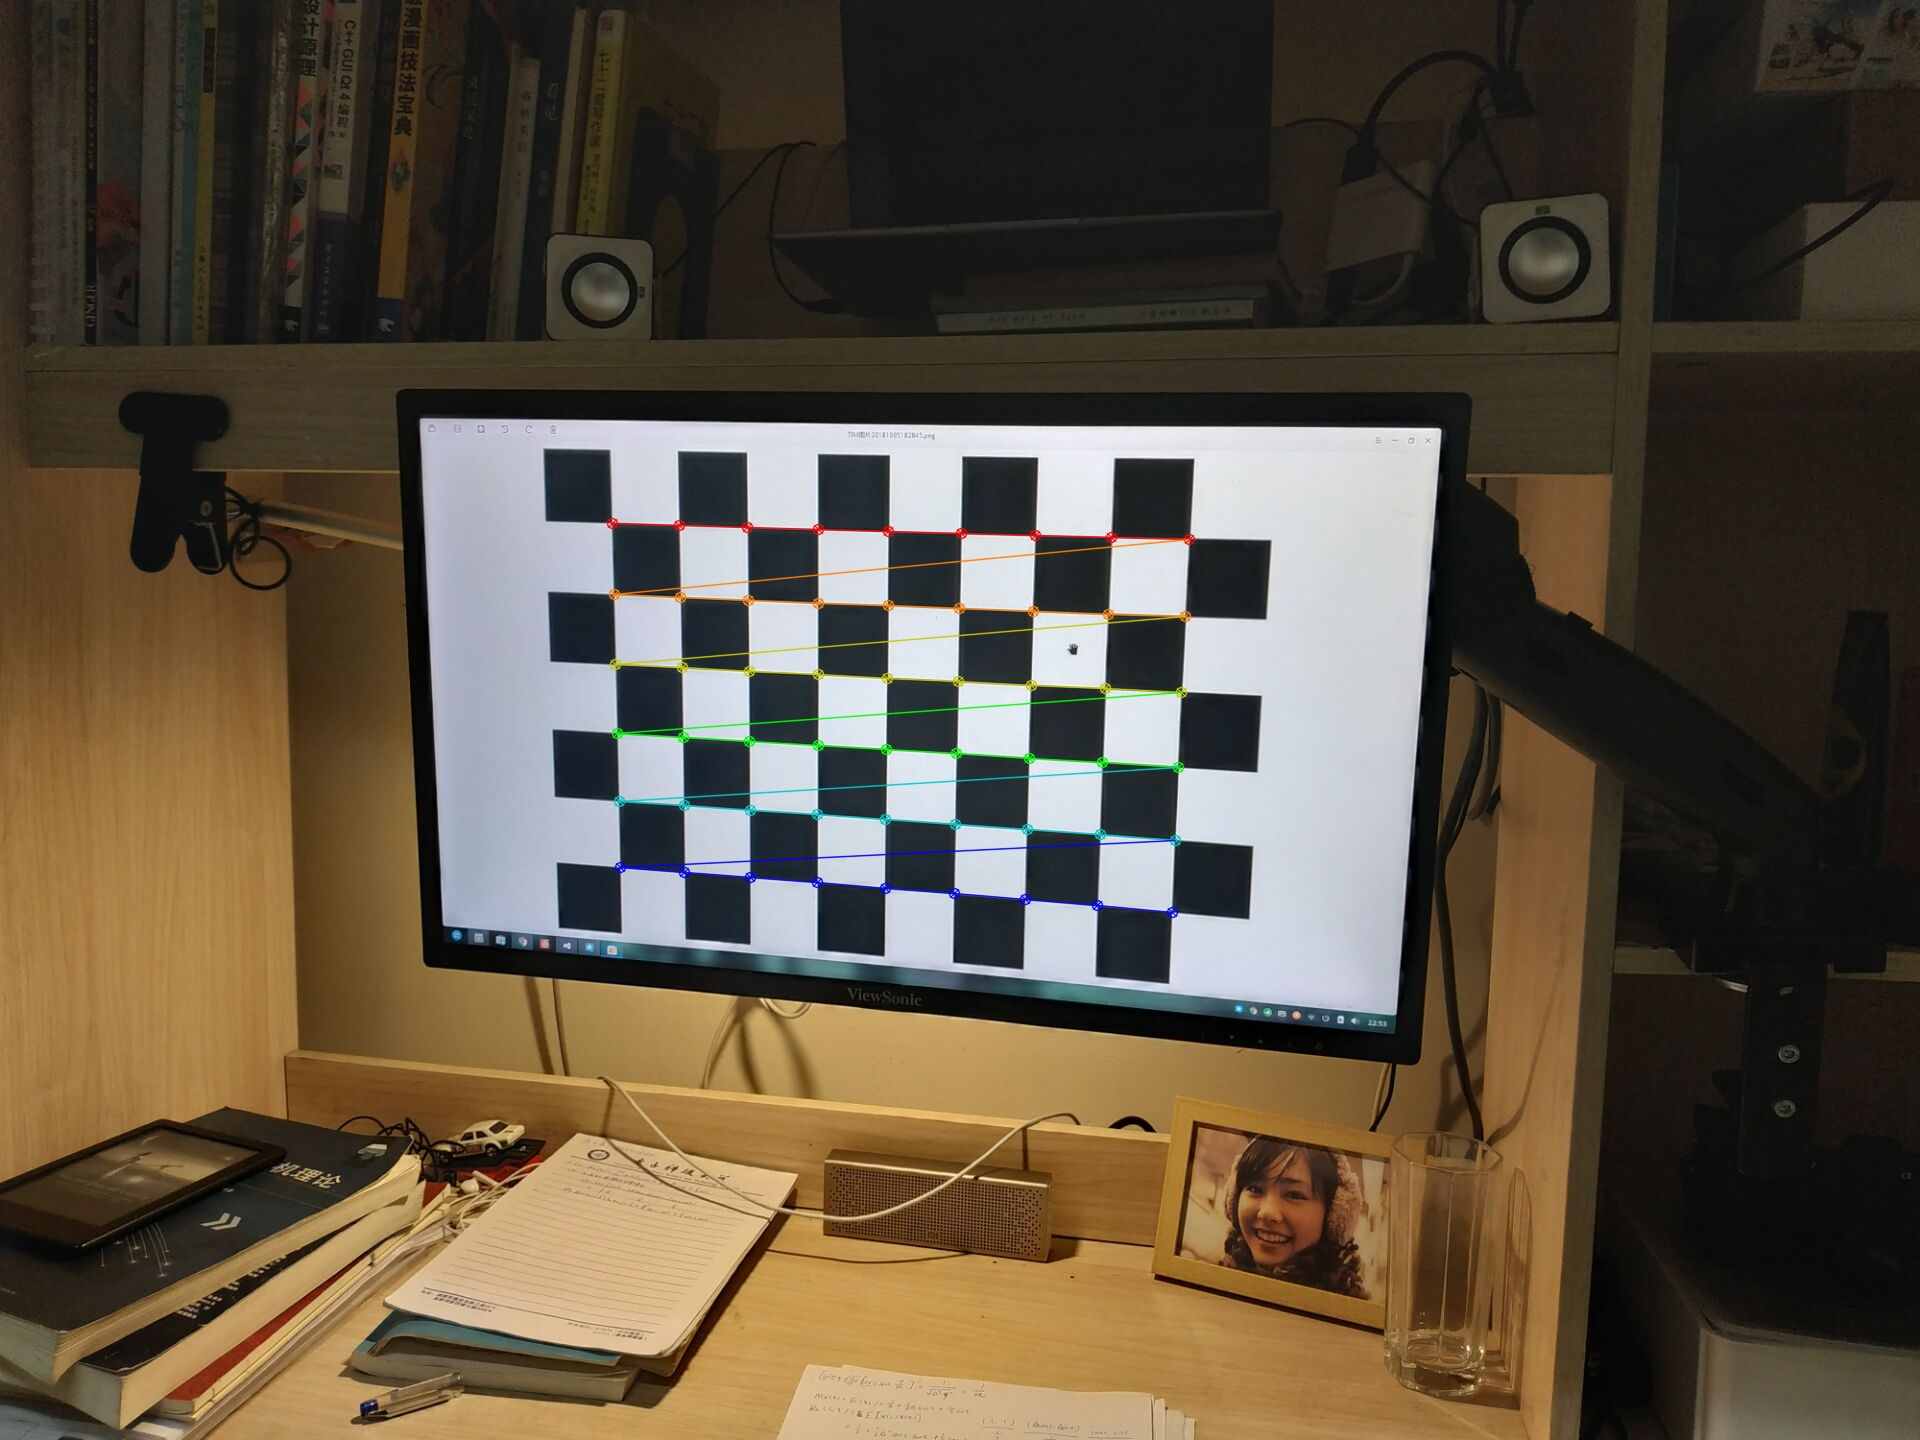
\includegraphics[width=6cm]{../code/images/2_jpg_with_corners.jpg}
        \end{minipage}

        \caption{左侧为原图,右侧为找出角点的图片}
        \label{fig1}
    \end{figure}

    图\ref{fig1}展示了角点的查找结果。

    \subsection{相机标定}
    利用上一步中找出的角点,便可以获得对应的Object Points和Image Points,然后便可以调用Opencv的标定函数进行标定,并获得了标定结果、内参矩阵、畸变系数、旋转矩阵和平移向量。本次实验得到的内参矩阵如下:

    \begin{equation}
        IntrinsicMatrix = \left[
        \begin{matrix}
            1.41569298e+03 & 0.00000000e+00 & 9.46418154e+02 \\
            0.00000000e+00 & 1.41306861e+03 & 7.21098480e+02 \\
            0.00000000e+00 & 0.00000000e+00 & 1.00000000e+00
        \end{matrix}
        \right]
    \end{equation}

    \subsection{去除畸变}
    上一步我们已经得到了相机内参和畸变系数,在将图像去畸变之前,我们还可以优化内参数和畸变系数,通过设定自由自由比例因子$\alpha$。当$\alpha$设为0的时候,将会返回一个剪裁过的将去畸变后不想要的像素去掉的内参数和畸变系数;当$\alpha$设为1的时候,将会返回一个包含额外黑色像素点的内参数和畸变系数,然后我们就可以使用新得到的内参数矩阵和畸变系数对图像进行去畸变了。

    \begin{figure}[htbp]
        \centering
        \begin{minipage}[t]{0.4\textwidth}
            \centering
            \includegraphics[width=6cm]{../code/test/0.jpg}
        \end{minipage}
        \begin{minipage}[t]{0.4\textwidth}
            \centering
            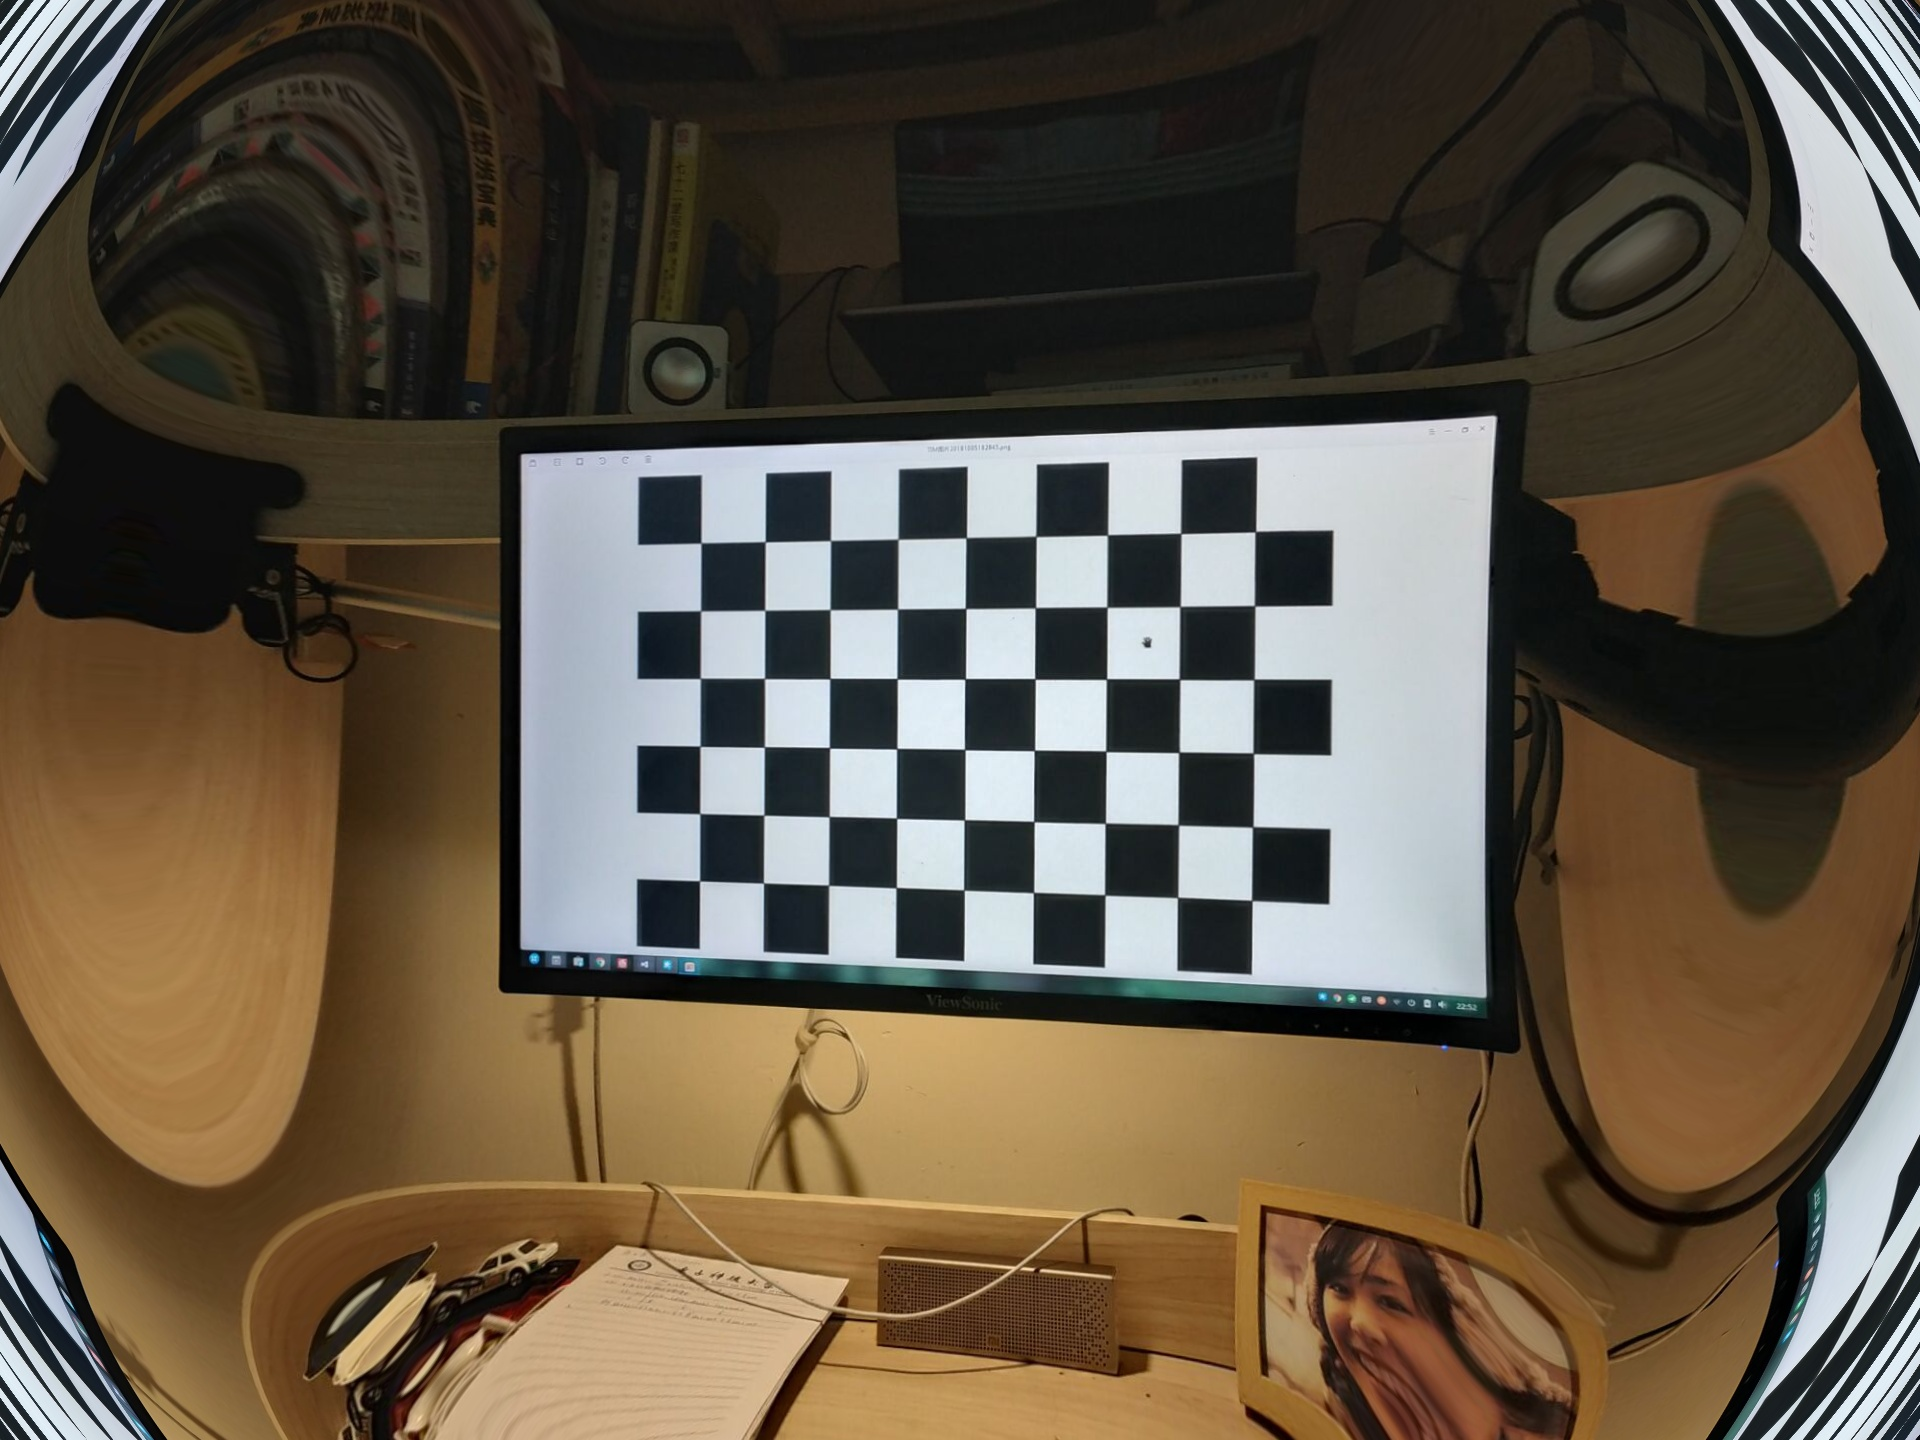
\includegraphics[width=6cm]{../code/test/0_jpg_undistorted.jpg}
        \end{minipage}

        \begin{minipage}[t]{0.4\textwidth}
            \centering
            \includegraphics[width=6cm]{../code/test/1.jpg}
        \end{minipage}
        \begin{minipage}[t]{0.4\textwidth}
            \centering
            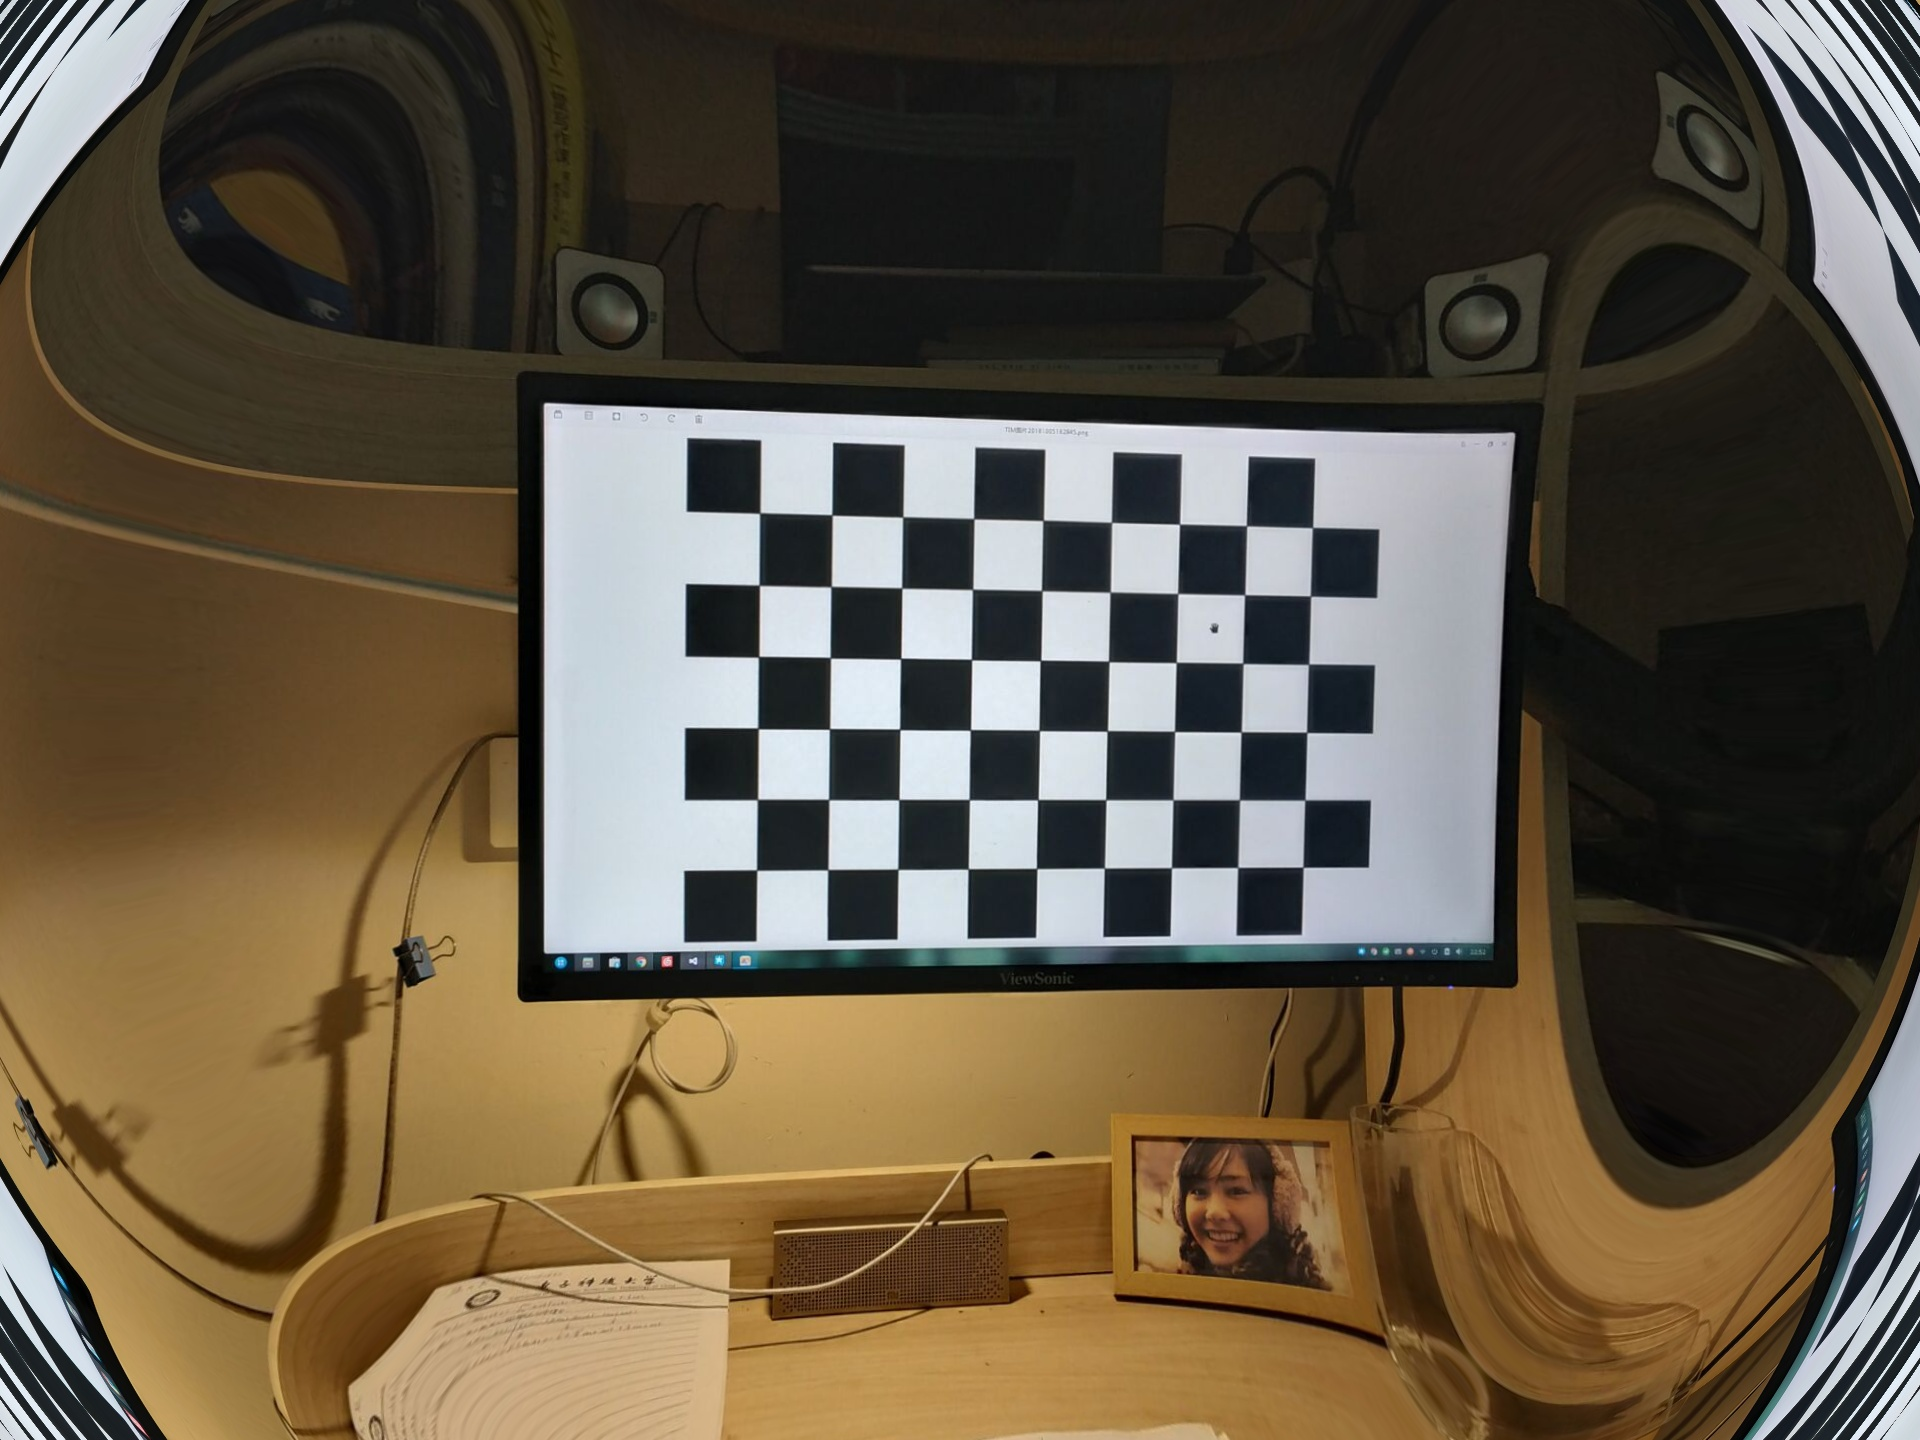
\includegraphics[width=6cm]{../code/test/1_jpg_undistorted.jpg}
        \end{minipage}

        \caption{左侧为原图,右侧为矫正畸变之后的图片}
        \label{fig2}
    \end{figure}

    图\ref{fig2}展示了去除畸变的效果,由于图片是采用手机拍摄,图片本身已经经过手机厂商的算法处理过了,所以畸变并不是特别明显。

    \subsection{计算误差}
    通过反投影误差,我们可以来评估结果的好坏。越接近0,说明结果越理想。通过之前计算的内参数矩阵、畸变系数、旋转矩阵和平移向量,使用cv2.projectPoints()计算三维点到二维图像的投影,然后计算反投影得到的点与图像上检测到的点的误差,最后计算一个对于所有标定图像的平均误差,这个值就是反投影误差。
    \begin{figure}[htbp]
        \centering
        \begin{minipage}[h]{0.4\textwidth}
            \centering
            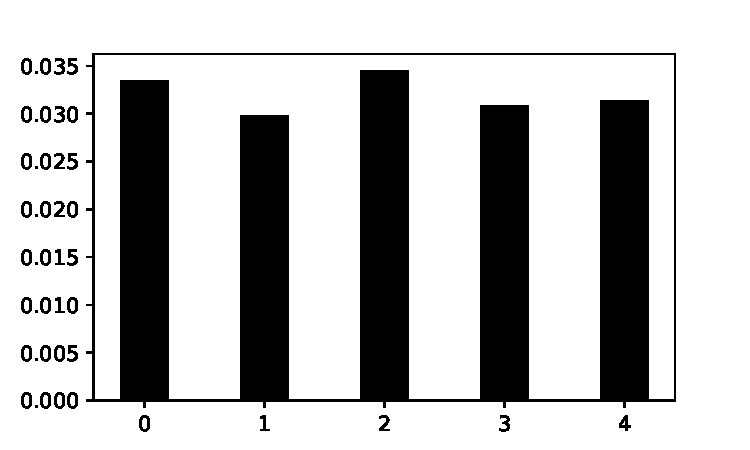
\includegraphics[width=6cm]{./errors.pdf}
        \end{minipage}
        \begin{minipage}[h]{0.4\textwidth}
            \centering
            \begin{tabular}{ll} %l(left)居左显示 r(right)居右显示 c居中显示
                \toprule
                序号 & 误差\\
                \midrule
                0 & 0.03345311519063753\\
                1 & 0.02976615118171713\\
                2 & 0.03452631311393804\\
                3 & 0.03087827628050186\\
                4 & 0.03141971741304798\\
                \midrule
                平均 & 0.032009\\
                \bottomrule
            \end{tabular}
        \end{minipage}
        \caption{标定图片的反投影误差}
    \end{figure}

    \section{附录}
        \begin{lstlisting}[language=Python]
import cv2
import numpy as np
import glob
import os
import matplotlib.pyplot as plt

def filter_word(string, words):
    '''
    Return True if string contains the word from array words.
    '''
    for word in words:
        if word in string:
            return True
    return False

root = __file__[0:__file__.rfind(os.sep)]

# 首先找到棋盘格角点
criteria = (cv2.TERM_CRITERIA_EPS + cv2.TERM_CRITERIA_MAX_ITER, 30, 0.001)
w, h = 9, 6 # 棋盘大小

points = np.zeros((w * h, 3), np.float32)
points[:, :2] = np.mgrid[0:w, 0:h].T.reshape(-1, 2)

object_points = [] # 世界坐标系的三维点
img_points = [] # 平面中的二维点

images = glob.glob(root + '/images/*')

for filename in images:
    if filter_word(filename, ['with_corners']):
        continue
    image = cv2.imread(filename)
    gray = cv2.cvtColor(image, cv2.COLOR_BGR2GRAY)
    # 搜索棋盘格点
    ret, corners = cv2.findChessboardCorners(gray, (w, h), None)
    if ret is True:
        cv2.cornerSubPix(gray, corners, (11, 11), (-1, -1), criteria)
        object_points.append(points)
        img_points.append(corners)
        # 显示角点
        cv2.drawChessboardCorners(image, (w, h), corners, ret)
        new_fileaname = filename.replace('.', '_') + '_with_corners.jpg'
        cv2.imwrite(new_fileaname, image)

# 开始相机标定
ret, mtx, dist, rvecs, tvecs = cv2.calibrateCamera(object_points, img_points,
    gray.shape[::-1], None, None)

for filename in glob.glob(root + '/test/*'):
    if filter_word(filename, ['undistorted']):
        continue
    # 去除畸变
    test_img = cv2.imread(filename)
    height, width = test_img.shape[:2]
    result = cv2.undistort(test_img, mtx, dist, None, mtx)
    cv2.imwrite(filename.replace('.', '_') + '_undistorted.jpg', result)

# 反投影误差
total_error = 0
errors = []
N = len(object_points)
for i in range(N):
    img_points2, _ = cv2.projectPoints(object_points[i], rvecs[i], tvecs[i],
        mtx, dist)
    error = cv2.norm(img_points[i], img_points2, cv2.NORM_L2) / len(img_points2)
    total_error += error
    errors.append(error)
mean_error = total_error / N

print('Mean error: %f' % mean_error)

# 绘制图表
plt.figure(figsize=(5, 3))
plt.bar(range(N), errors, width=0.4, color='black')
plt.savefig(root.replace('code', '') + 'doc/errors.pdf')
        \end{lstlisting}

    \end{document}